\chapter{Background and Related Work}
\label{ch:background}

This chapter presents background information on the field of edge computing
(\cref{sec:bg-edge}), the SteelEagle autonomous drone system
(\cref{sec:steeleagle-bg}), and the OODA loop framework (\cref{sec:ooda-loop}).

\section{Edge Computing}
\label{sec:bg-edge}

There has been a huge increase in the number of mobile and Internet of Things
(IoT) devices in recent years, driven by advancements in sensor, networking,
and processing technologies.  These innovations have made devices smaller, more
affordable, and more versatile, enabling their integration into nearly every
aspect of modern life. As explained in \cref{sec:overview}, despite the
innovations, these mobile devices remain resource-poor relative to static
resources. A wearable device like a smartwatch, for example, has limited
battery life, which constraints its ability to sustain prolonged conversation
with an onboard AI virtual assistant. In 1997, Noble et al extended an adaptive
application-aware framework called Odyssey, which provides remote data access
to mobile clients, to perform speech recognition on a resource-constrained
mobile device by offloading compute to a remote server \cite{noble1997}. This
offloading technique allows a mobile device to circumvent its resource
limitations.

But a key question remains---where to offload? The cloud is an
appealing choice today because of its on-demand and scalable nature. However,
cloud computing resources are consolidated into datacenters at a small number
of geographic locations to leverage economies of scale, increasing the distance
between ends users and the cloud and thus increasing network latency. This can
be a dealbreaker for latency-sensitive interactive applications such as
augmented reality. An emperical study conducted with 2,504 Amazon EC2 clients
found that more than 60\% of the clients experienced latencies higher than 40
ms \cite{choy2012}. However, immersive augmented reality on a wearable device
has a latency bound of 16 milliseconds \cite{ellis2004}.
To attain crisp interactive application response,
Satyanarayanan et al introduced the novel paradigm of edge computing
\cite{satya2009}.


Edge computing is a paradigm in which substantial computing and storage
resources---referred to as "cloudlets"---are situated at the edge of the
Internet in close proximity to mobile devices, sensors, end users, and Internet
of Things (IoT) devices. This proximity offers several key advantages \cite{satya2017}:
\begin{itemize}
    \item It allows offloading to truly shine, enabled by the low latency, high
bandwidth, and low jitter links to the cloudlets
    \item It reduces the bandwidth demand that IoT devices like video cameras place on the cloud, thus increasing scalability \cite{premsankar2018}
    \item A cloudlet can enforce a user's privacy policies specified for their IoT sensor data before the extracted information and metadata obtained from it is sent to the cloud
    \item Cloudlets help mitigate cloud outages by serving as a fallback service
\end{itemize}

\section{SteelEagle Autonomous Drone System}
\label{sec:steeleagle-bg}

\begin{figure}[htbp]
\centering
\begin{subfigure}[t]{0.3\textwidth}
\centering
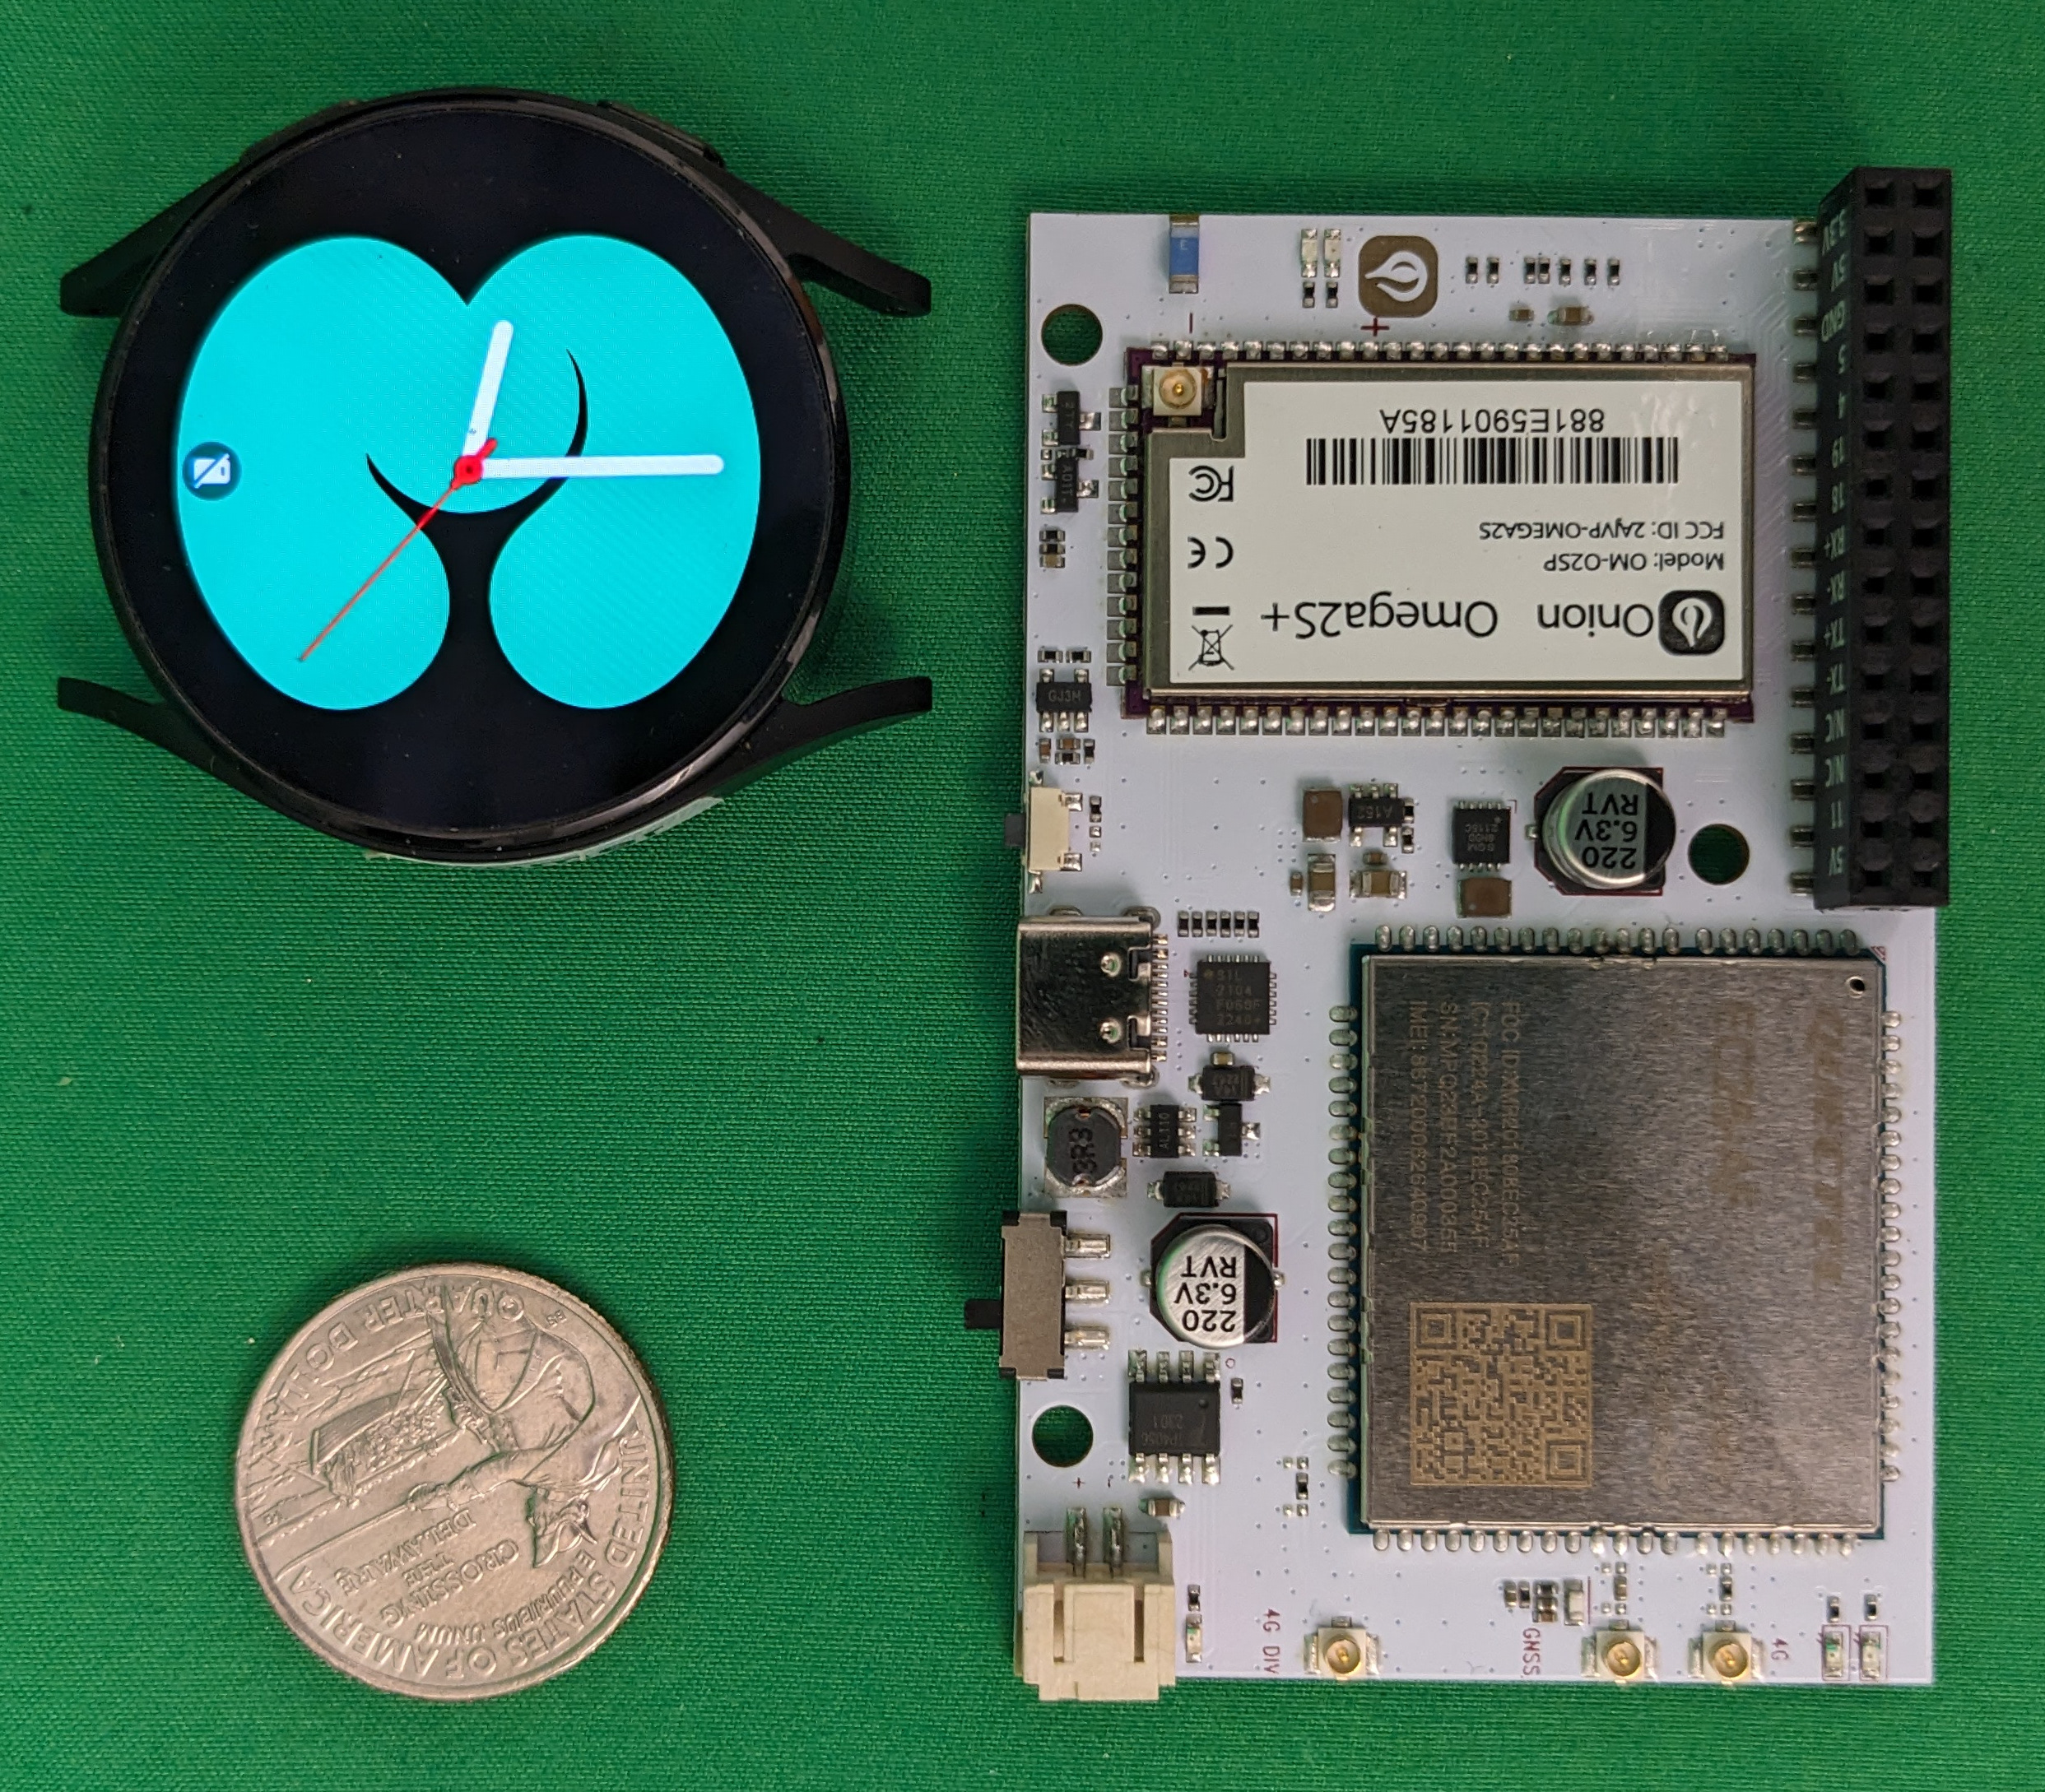
\includegraphics[height=1.6in]{sec2023-figs/fig-omega-internals.jpg}\\
\caption{The Samsung Galaxy Watch and the Onion Omega 2 LTE}
\end{subfigure}
\hspace{3em}
\begin{subfigure}[t]{0.3\textwidth}
\centering
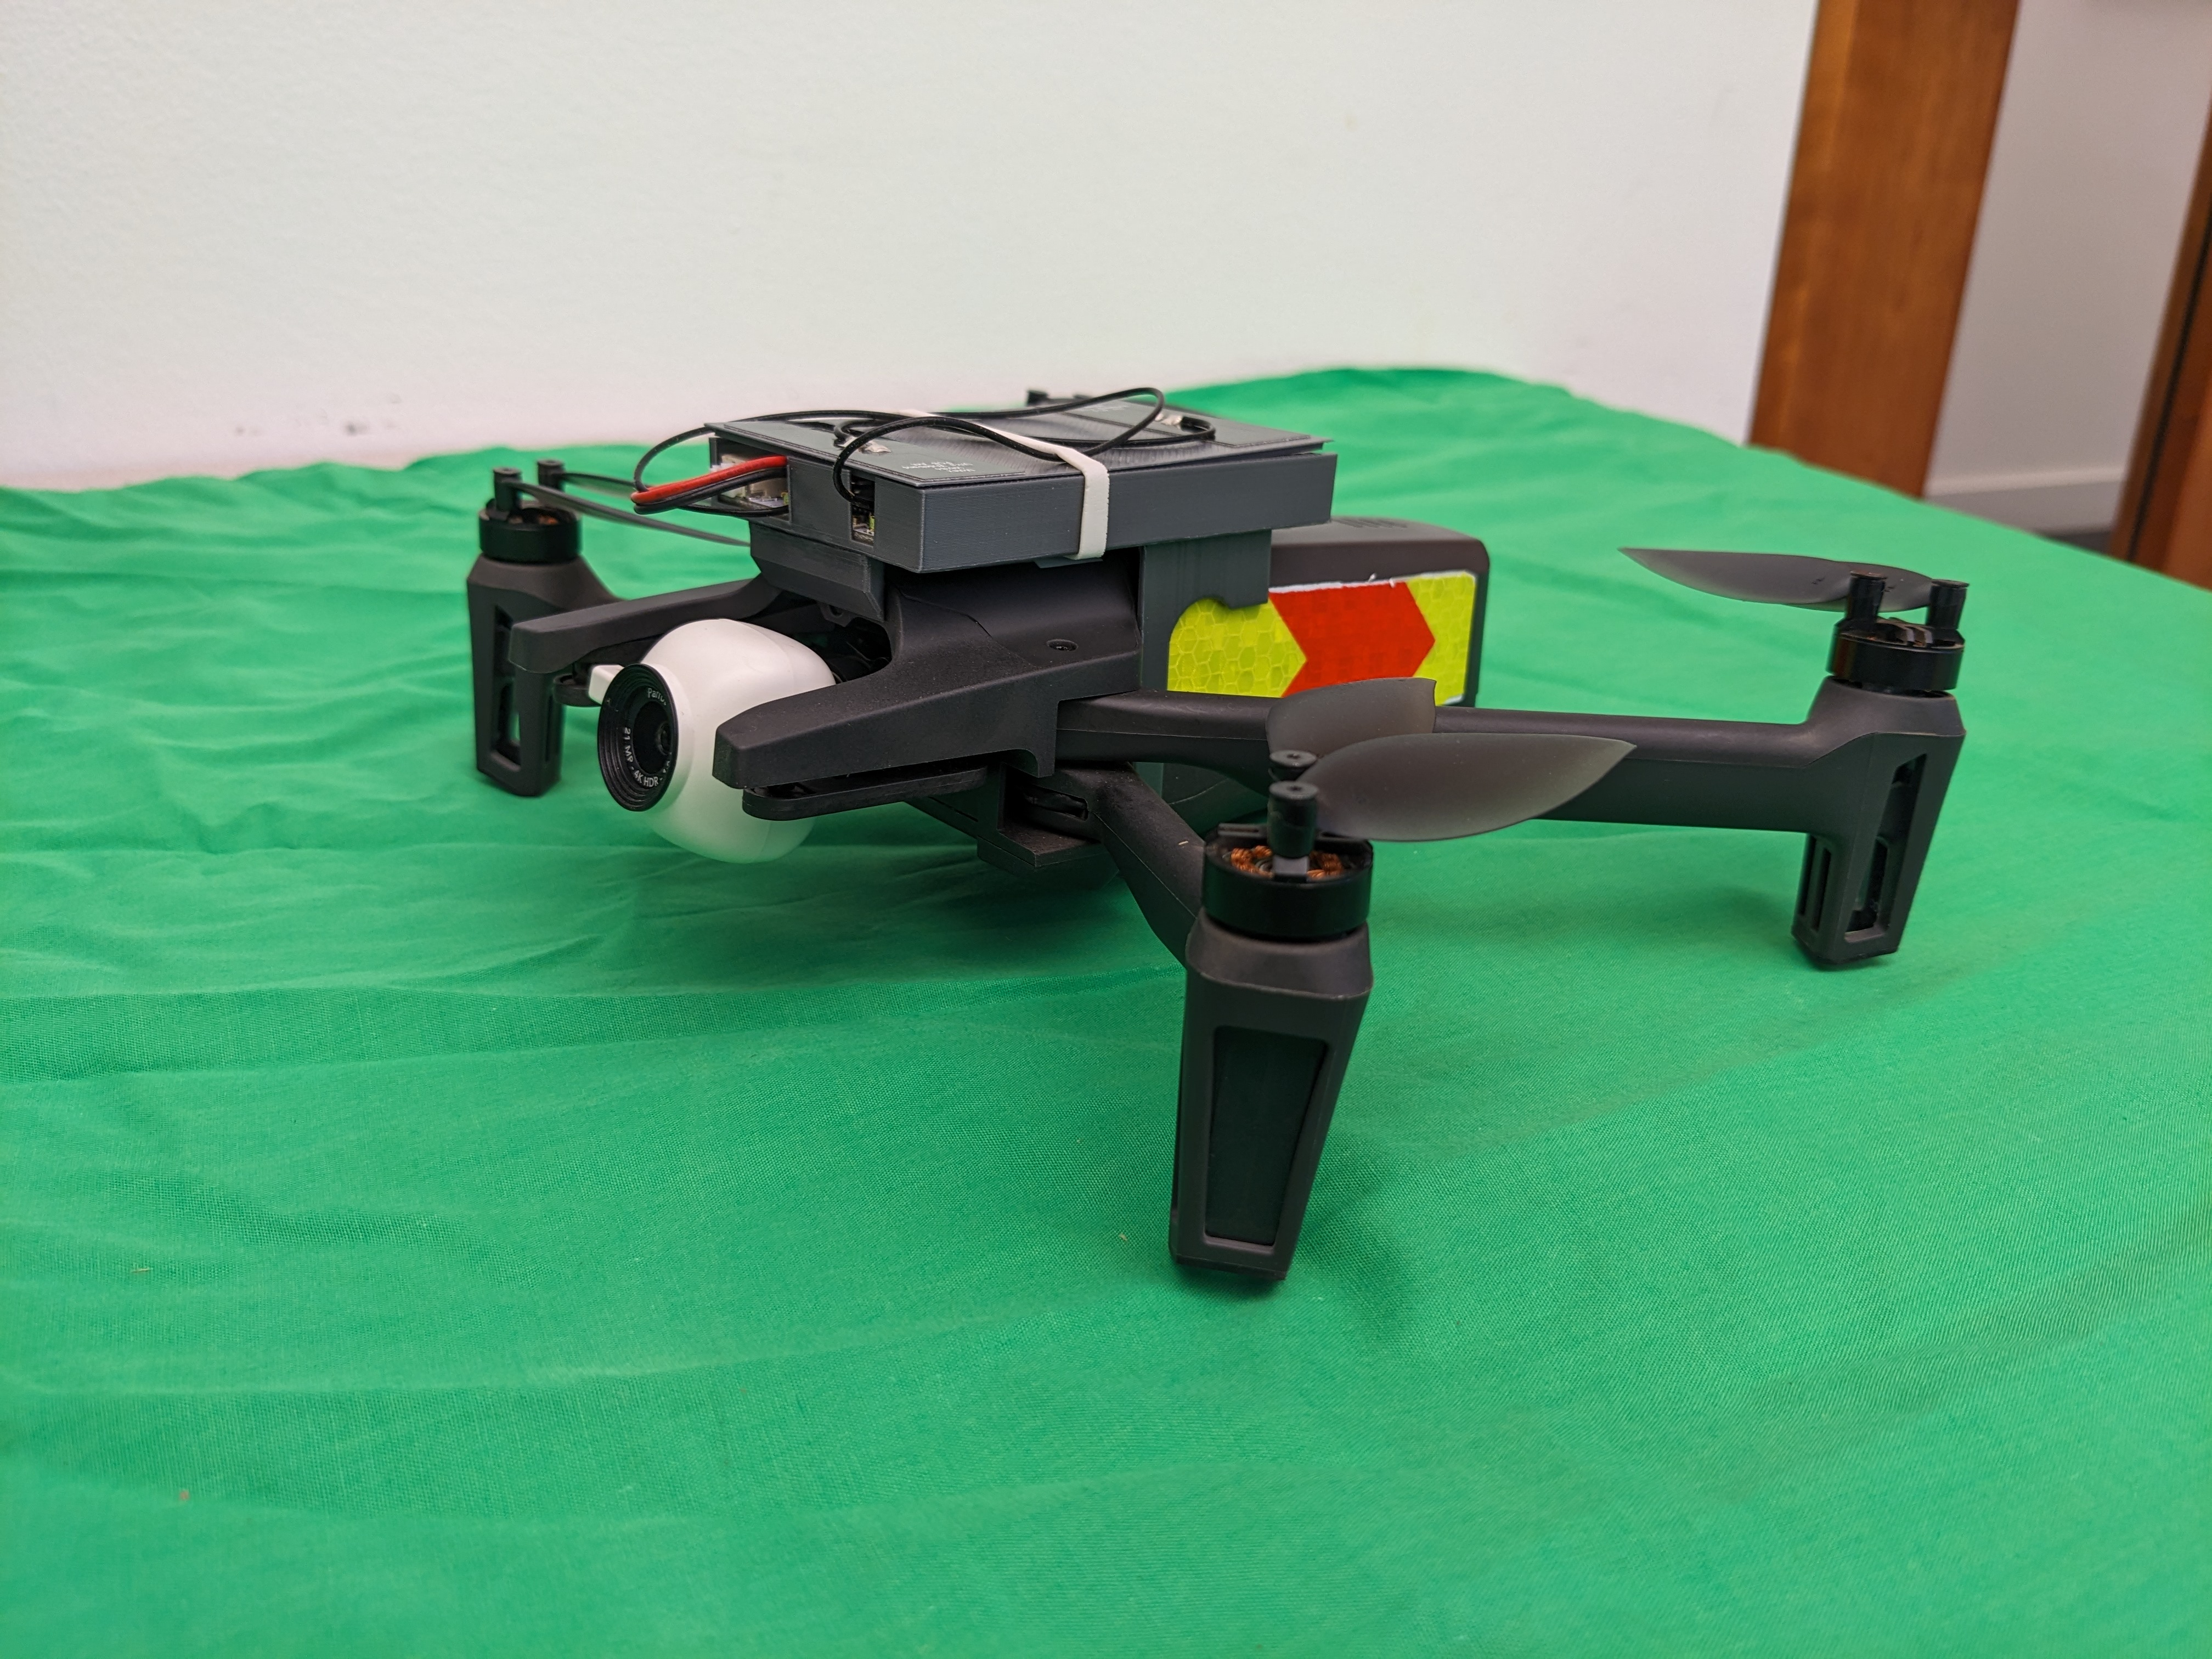
\includegraphics[height=1.6in]{sec2023-figs/fig-omega-harness.jpg}
\caption{Onion Omega 2 LTE mounted on Parrot Anafi}
\end{subfigure}
\caption{The Hardware Used in SteelEagle (from Bala et al \cite{bala2024})}
\label{fig:galaxy_watch}
\end{figure}

Autonomous drones perform tasks such as navigating between waypoints and
tracking moving objects without the need for a human pilot.  However,
autonomous drones today are large and expensive. Lightweight drones are more
appealing, as they present a smaller public safety hazard and thus face fewer
regulations. The FAA, for instance, has pre-authorized flights over people and
vehicles by drones weighing less than 250 g. On the other hand, cheaper drones
will help accelerate the uptake of autonomous drones in scenarios that stand to
benefit the most from their abilities. Search and rescue operations, as well as
wildlife conservation efforts that involve monitoring wildlife populations,
will benefit immensely from the abilities of drones to cover large areas
quickly. The potential for good increases exponentially with a swarm of drones
working cooperatively \cite{scherer2015}. In rural areas with limited law
enforcement resources, for instance, a swarm of drones could quickly scan
large swathes of land looking for an abducted child.

Over time, autonomous drones will
become cheaper and lighter as new ASIC designs are developed that are more
energy efficient and mass production lowers costs. Until then, leveraging edge
computing to add autonomous features to lighter consumer-grade drones at a much
lower price tag is a very appealing proposition. This is the software-hardware
co-evolution path that Satyanarayanan et al outlined, presenting offloading as
a way to "cheat" until ASIC designs are available \cite{satya21}.

Bala et al \cite{bala2024} have demonstrated that even drones with a monocular
camera can perform tasks such as object tracking and depth inference
reasonablly well. In their setup, Bala et al initially used a Samsung Galaxy
smartwatch as a communications relay, mounted on top of a Parrot Anafi drone,
for a total takeoff weight of about 360 g. The Samsung Galaxy smartwatch is
appealing because it is an enclosed system, including a battery and an
enclosure protected from the elements. It also has the ability to run Android
applications onboard.  However, the constant LTE tranmission on the watch
caused it to hit its thermal limits, set so that the watch can be safely worn
on the human wrist, and shut down. \Cref{fig:watch-themal-curve} shows the
increase in temperature of the watch for a frame rate of 0.7 and 2.

As a result, the Samsung Galaxy smartwatch
could sustain a very low frame rate.

\begin{figure}[htbp]
\centering
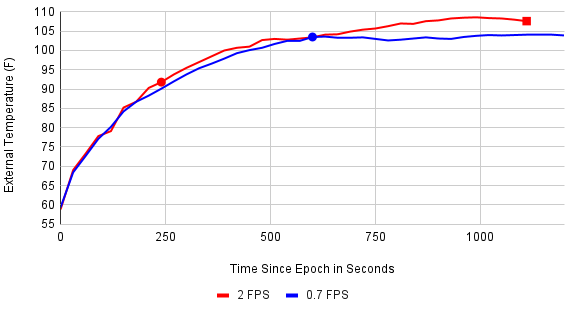
\includegraphics[width=0.6\textwidth]{sec2023-figs/fig-thermal-curve.png}
\caption{The Samsung Galaxy Payload Thermal Curve (from Bala et al \cite{bala2024})}
\label{fig:watch-themal-curve}
\end{figure}

As an alternative, Bala et al used the Onion Omega 2 system-on-a-chip device
\cite{onionomega2}. While the Omega 2 does not have the thermal limitations
present in the Galaxy smartwatch, it has very weak computational capabilities.
Intended for use as an IoT module, the Omega 2 runs the 580MHz MIPS 24KEc CPU
and has only 16 MB of flash storage. In the SteelEagle setup, a VPN tunnel
between the cloudlet and the Omega 2 over 4G LTE cellular allows communication
with the drone that is connected to the Omega 2 over Wi-Fi. The Omega 2's role
is to route packets between its Wi-Fi and LTE network interfaces, truly acting
as just a communications relay.

\section{OODA Loop Framework}
\label{sec:ooda-loop}

\begin{figure}[htbp]
\centering
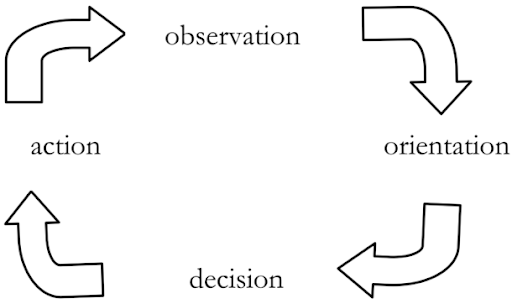
\includegraphics[width=0.4\textwidth]{figs/ooda-loop.png}
\caption{The OODA Loop}
\label{fig:ooda-loop}
\end{figure}

The "Observe, Orient, Decide, Act" (OODA) loop framework devised by military
strategist John R. Boyd provides a framework to structure our investigation
into the end-to-end latency of SteelEagle. It consists of four stages:

\begin{itemize}
    \item \textbf{Observe.} Involves obtaining new information about the environment
    \item \textbf{Orient.} Analysis and interpretation of the obtained information
    \item \textbf{Decide.} Choosing a course of action
    \item \textbf{Act.} Execution of the chosen action
\end{itemize}

According to Boyd, decision-making happens in a continuous iteration of these
steps. Boyd attributed the faster OODA loop of U.S. pilots flyng F-86s, because
of the bubble-shaped canopy offering better visibility and hydraulic controls
that allowed for easier switching between manoeuvres, as the reason the slower
F-86s fared better than the North Korean MiG-15s during the Korean War
\cite{morton1995}. In the context of autonomous drones, a drone with a tighter
OODA loop corresponds to a more agile drone. It means that the drone is able
to react faster to changes in its environment.

Instead of measuring just the overall system latency, performing a
break down of the latency across the OODA steps provides more insight into
system latency bottlenecks.

\begin{comment}
\section{Background: SteelEagle Benchmarks}
Bala et al performed experiments to measure the agility of the SteelEagle
system. The experiment setup involves setting up a stationary drone in a lab
setting, with its camera pointed at a display connected to the cloudlet, showing
the current timestamp in milliseconds. The drone camera captures images of this
timestamp and transmits them to the cloudlet through the SteelEagle pipeline.
\end{comment}
